% ══════════════════════════════════════════════════════════════════════════════
%  AMR Prediction System — Project Report
%  Compile on Overleaf (pdfLaTeX). Upload rgukt.jpeg alongside this file.
% ══════════════════════════════════════════════════════════════════════════════
\documentclass[12pt,a4paper]{report}

% ── Encoding & Fonts ──────────────────────────────────────────────────────────
\usepackage[T1]{fontenc}
\usepackage[utf8]{inputenc}
\usepackage{lmodern}

% ── Page Layout ───────────────────────────────────────────────────────────────
\usepackage[a4paper,
            top=1.3in, bottom=1.3in,
            left=1.2in, right=1.2in]{geometry}

% ── Graphics ──────────────────────────────────────────────────────────────────
\usepackage{graphicx}
\usepackage{eso-pic}

% ── TikZ ──────────────────────────────────────────────────────────────────────
\usepackage{tikz}
\usetikzlibrary{shapes.geometric, arrows.meta, positioning,
                fit, backgrounds, calc}

% ── Math ──────────────────────────────────────────────────────────────────────
\usepackage{amsmath}
\usepackage{amssymb}

% ── Tables ────────────────────────────────────────────────────────────────────
\usepackage{booktabs}
\usepackage{longtable}
\usepackage{array}
\usepackage{multirow}
\usepackage{tabularx}
\usepackage{rotating}

% ── Colors ────────────────────────────────────────────────────────────────────
\usepackage{xcolor}
\definecolor{rguktblue}{RGB}{0,60,120}
\definecolor{rguktgold}{RGB}{180,130,0}
\definecolor{darkblue}{RGB}{0,40,100}
\definecolor{darkgray}{RGB}{80,80,80}
\definecolor{codegreen}{rgb}{0,0.52,0}
\definecolor{codegray}{rgb}{0.45,0.45,0.45}
\definecolor{codeblue}{rgb}{0,0.2,0.7}
\definecolor{codeback}{rgb}{0.97,0.97,0.97}

% ── Code Listings ─────────────────────────────────────────────────────────────
\usepackage{listings}
\lstset{
  backgroundcolor=\color{codeback},
  basicstyle=\footnotesize\ttfamily,
  keywordstyle=\color{codeblue}\bfseries,
  commentstyle=\color{codegreen}\itshape,
  numberstyle=\tiny\color{codegray},
  stringstyle=\color{red!65!black},
  breaklines=true,
  numbers=left,
  numbersep=6pt,
  frame=single,
  rulecolor=\color{gray!35},
  captionpos=b,
  showstringspaces=false,
  tabsize=2,
}

% ── Algorithm ─────────────────────────────────────────────────────────────────
\usepackage[ruled,vlined,linesnumbered]{algorithm2e}
\SetKwInput{KwInput}{Input}
\SetKwInput{KwOutput}{Output}

% ── Headers / Footers ─────────────────────────────────────────────────────────
\usepackage{fancyhdr}
\pagestyle{fancy}
\fancyhf{}
\fancyhead[L]{\small\textcolor{rguktblue}{\textit{Multi-Drug AMR Prediction System}}}
\fancyhead[R]{\small\textcolor{rguktblue}{\thepage}}
\fancyfoot[C]{\small\textcolor{rguktgold}{RGUKT\,---\,Department of Computer Science \& Engineering}}
\renewcommand{\headrulewidth}{0.5pt}
\renewcommand{\footrulewidth}{0.5pt}

% ── Chapter / Section Titles ──────────────────────────────────────────────────
\usepackage{titlesec}
\titleformat{\chapter}[display]
  {\normalfont\huge\bfseries\color{rguktblue}}
  {\chaptertitlename~\thechapter}{8pt}{\Huge}
\titlespacing*{\chapter}{0pt}{0pt}{18pt}
\titleformat{\section}{\large\bfseries\color{darkblue}}{\thesection}{1em}{}
\titleformat{\subsection}{\normalsize\bfseries\color{darkblue}}{\thesubsection}{1em}{}

% ── Hyperlinks ────────────────────────────────────────────────────────────────
\usepackage{hyperref}
\hypersetup{
  colorlinks=true,
  linkcolor=rguktblue,
  urlcolor=codeblue,
  citecolor=rguktgold,
  bookmarks=true,
  pdfpagemode=UseOutlines,
}

% ── Spacing ───────────────────────────────────────────────────────────────────
\usepackage{setspace}
\onehalfspacing

% Rename Bibliography → References in report class
\renewcommand{\bibname}{References}

% ── Captions ──────────────────────────────────────────────────────────────────
\usepackage{caption}
\captionsetup{font=small, labelfont={bf,color=rguktblue}, margin=10pt}

% ── Lists ─────────────────────────────────────────────────────────────────────
\usepackage{enumitem}

% ── tcolorbox (info boxes) ────────────────────────────────────────────────────
\usepackage{tcolorbox}
\tcbuselibrary{skins,breakable}
\tcbset{
  infobox/.style={
    colback=blue!4, colframe=rguktblue, boxrule=0.7pt,
    arc=3pt, fonttitle=\bfseries\small\color{rguktblue},
    left=6pt, right=6pt, top=4pt, bottom=4pt,
  }
}

% ════════════════════════════════════════════════════════════════════════════
%  DOUBLE BORDER ON EVERY PAGE  (blue outer  +  gold inner)
% ════════════════════════════════════════════════════════════════════════════
\AddToShipoutPictureBG{%
  \begin{tikzpicture}[remember picture, overlay]
    \draw[rguktblue, line width=2.8pt]
      ([xshift=12pt,  yshift=-12pt] current page.north west) rectangle
      ([xshift=-12pt, yshift= 12pt] current page.south east);
    \draw[rguktgold, line width=0.9pt]
      ([xshift=17pt,  yshift=-17pt] current page.north west) rectangle
      ([xshift=-17pt, yshift= 17pt] current page.south east);
  \end{tikzpicture}%
}

% ════════════════════════════════════════════════════════════════════════════
\begin{document}

% ────────────────────────────────────────────────────────────────────────────
%  TITLE PAGE
% ────────────────────────────────────────────────────────────────────────────
\begin{titlepage}
\thispagestyle{empty}
\begin{center}

  \includegraphics[width=3.8cm]{rgukt.jpeg}\\[0.3cm]
  {\Large\bfseries\color{rguktblue}
    Rajiv Gandhi University of Knowledge Technologies}\\[0.1cm]
  {\normalsize\color{darkblue} RGUKT -- Nuzvid, Andhra Pradesh -- 521202}\\[0.08cm]
  {\normalsize\bfseries Department of Computer Science \& Engineering}\\[0.35cm]

  \noindent\rule{\linewidth}{1.2pt}\\[0.15cm]
  {\large\bfseries\color{rguktgold} B.Tech Mini Project Report}\\[0.15cm]
  \noindent\rule{\linewidth}{1.2pt}\\[0.45cm]

  % Project Title
  {\fontsize{22}{26}\selectfont\bfseries\color{rguktblue} Multi-Drug AMR Prediction System}\\[0.25cm]
  {\LARGE\bfseries\color{darkblue}
    Machine Learning Approach for Predicting\\[0.15cm]
    Antimicrobial Resistance}\\[0.3cm]
  {\normalsize\itshape\color{darkgray}
    ``Predicting Sensitive and Resistant Profiles based on Clinical Features''}\\[0.7cm]

  % Guide
  {\large\bfseries Under the Guidance of}\\[0.3cm]
  {\large\bfseries Mr.~Kumar Anurupam~MS}\\[0.1cm]
  {\normalsize Assistant Professor (C), Dept. of CSE, RGUKT}\\[0.6cm]

  {\normalsize\bfseries Academic Year: 2025 -- 2026}

\end{center}
\end{titlepage}

% ────────────────────────────────────────────────────────────────────────────
%  CERTIFICATE
% ────────────────────────────────────────────────────────────────────────────
\chapter*{Certificate}
\addcontentsline{toc}{chapter}{Certificate}
\thispagestyle{fancy}

This is to certify that the project entitled \textbf{``Multi-Drug AMR Prediction System''} submitted by the following students is the bonafide work carried out under our supervision, in partial fulfilment of the requirements for the award of the B.Tech degree in Computer Science \& Engineering at Rajiv Gandhi University of Knowledge Technologies, RGUKT -- Nuzvid, during the academic year 2025--2026.

\vspace{0.5cm}
\noindent\textbf{Students:}\\[0.2cm]
\renewcommand{\arraystretch}{1.4}
\begin{tabular}{@{}p{5.5cm}p{2cm}p{4cm}@{}}
  \textbf{Name:} Pedda Nithin Kumar        & \textbf{ID No:} & N210171 \\
  \textbf{Name:} Pitti Sunil Kumar        & \textbf{ID No:} & N211000 \\
  \textbf{Name:} Teela Vijayalakshmi       & \textbf{ID No:} & N210710 \\
  \textbf{Name:} Samireddy Nikhila     & \textbf{ID No:} & N210529 \\
\end{tabular}

\vspace{1.2cm}
\noindent
\begin{tabular}{@{}p{7cm}p{7cm}@{}}
  \textbf{Project Guide}               & \textbf{Head of Department}         \\[0.6em]
  \underline{\hspace{5.5cm}}           & \underline{\hspace{5.5cm}}          \\[0.2em]
  Mr. Kumar Anurupam MS                & Mr. A. Udaya Kumar M.Tech           \\
  Asst. Prof. (C), Dept. of CSE       & Asst. Prof., Dept. of CSE, RGUKT    \\
\end{tabular}

% ────────────────────────────────────────────────────────────────────────────
%  DECLARATION
% ────────────────────────────────────────────────────────────────────────────
\chapter*{Declaration}
\addcontentsline{toc}{chapter}{Declaration}
\thispagestyle{fancy}

We hereby declare that the project entitled \textbf{``Multi-Drug AMR Prediction System''} submitted in partial fulfilment of the requirements for the award of the degree of Bachelor of Technology in Computer Science \& Engineering at Rajiv Gandhi University of Knowledge Technologies, RGUKT -- Nuzvid, is a bonafide record of our original work carried out under the supervision of \textbf{Mr. Kumar Anurupam MS}.

We further declare that the work reported in this project has not been submitted and will not be submitted, either in part or in full, for the award of any other degree or diploma in this or any other institute or university.

\vspace{2cm}
\noindent
\renewcommand{\arraystretch}{1.7}
\begin{tabular}{@{}p{6.5cm}p{6.5cm}@{}}
  \textbf{P Nithin Kumar} (N210171)      & Signature: \underline{\hspace{3.5cm}} \\
  \textbf{P. Sunil Kumar} (N211000)      & Signature: \underline{\hspace{3.5cm}} \\
  \textbf{T Vijayalakshmi} (N210710)     & Signature: \underline{\hspace{3.5cm}} \\
  \textbf{Nikhila Samireddy} (N210529)   & Signature: \underline{\hspace{3.5cm}} \\
\end{tabular}

\vspace{1cm}
\noindent Place: \underline{\hspace{0.15cm}Nuzvid} \qquad Date:  \underline{\hspace{0.10cm} 09-04-2026}

% ────────────────────────────────────────────────────────────────────────────
%  ACKNOWLEDGEMENT
% ────────────────────────────────────────────────────────────────────────────
\chapter*{Acknowledgement}
\addcontentsline{toc}{chapter}{Acknowledgement}
\thispagestyle{fancy}

We express our sincere gratitude to our project guide \textbf{Mr. Kumar Anurupam MS}, Assistant Professor (C), Department of Computer Science and Engineering, RGUKT-Nuzvid, for his invaluable guidance, continuous encouragement, and constructive feedback throughout the project.

We are grateful to \textbf{Mr. A. Udaya Kumar M.Tech}, Head of the Department of CSE, RGUKT-Nuzvid, for providing the necessary infrastructure and facilities.

We also thank the \textbf{open-source community} behind the Python ecosystem, including the scikit-learn, PyTorch, and FT-Transformer maintainers — this project would not be possible without their contributions.

Finally, we thank our family and friends for their constant support and motivation.

% ────────────────────────────────────────────────────────────────────────────
%  ABSTRACT
% ────────────────────────────────────────────────────────────────────────────
\chapter*{Abstract}
\addcontentsline{toc}{chapter}{Abstract}
\thispagestyle{fancy}

Antimicrobial Resistance (AMR) is a significant global health threat that reduces the efficacy of antibiotics and complicates the treatment of infectious diseases. The conventional laboratory process of evaluating microbial susceptibility to various antibiotics is time-consuming. \textbf{The Multi-Drug AMR Prediction System} addresses this challenge by utilizing machine learning and deep learning to instantly predict resistance (R) and sensitivity (S) patterns for multiple drugs concurrently based on both microbial and patient clinical data.

The system incorporates dual operating modes. In \textit{Single Drug Mode}, a Random Forest Classifier is trained specifically for a single antibiotic. In \textit{Multi Drug Mode}, the system employs a MultiOutputClassifier and the state-of-the-art FT-Transformer to ascertain holistic cross-drug correlation patterns, identifying the optimal drug with the lowest resistance probability. The architecture encompasses a Flask-based RESTful API integrated with a dynamic, user-friendly frontend to render immediate clinical suggestions.

Evaluated over standard classification performance metrics including Accuracy, Precision, Recall, and Hamming Loss, the project successfully captures correlations between different comorbidities (such as Hypertension and Diabetes), patient demographic features, and antibiotic resistance patterns.

\vspace{0.5em}
\noindent\textbf{Keywords:} Antimicrobial Resistance (AMR), Multi-Label Classification, Random Forest, FT-Transformer, Flask Backend, Precision Medicine.

% ────────────────────────────────────────────────────────────────────────────
%  TABLE OF CONTENTS
% ────────────────────────────────────────────────────────────────────────────
\tableofcontents
\thispagestyle{fancy}
\listoffigures
\thispagestyle{fancy}
\listoftables
\thispagestyle{fancy}

% ════════════════════════════════════════════════════════════════════════════
%  CHAPTER 1 — INTRODUCTION
% ════════════════════════════════════════════════════════════════════════════
\chapter{Introduction}
\thispagestyle{fancy}

\section{Motivation}

Antimicrobial resistance occurs when bacteria, viruses, fungi, and parasites evolve over time and no longer respond to medicines, making infections more difficult to treat and increasing the risk of disease propagation, serious ailments, and death. Currently, clinical decision-making relies largely on laboratory cultures that require varying times (often 24-72 hours) to yield full resistance profiles.

Two primary challenges currently limit the timely response to microbial infections:

\begin{itemize}[noitemsep, leftmargin=*]
  \item \textbf{High Turnaround Times in Laboratories:} Prolonged in-vitro processes severely delay the administration of targeted antibiotic therapy, frequently leading clinicians to prescribe broad-spectrum antibiotics empirically, thereby inadvertently fueling further resistance.
  \item \textbf{Ignorance of Patient-Level Clinical Correlates:} Many predictive AMR systems focus purely on microbial genomic factors, failing to account for critical patient demographics (e.g., Age, Gender) or comorbidities (e.g., Hypertension, Diabetes), which possess significant correlations with resistance rates due to historical exposure to medication and differing immune capacities.
\end{itemize}

The core operational objective of this project may thus be specified:

\begin{tcolorbox}[infobox, title=Core Research Problem]
  How can machine learning models rapidly predict multi-drug susceptibility profiles (Sensitive/Resistant) by integrating both microbial data and patient clinical features to suggest an optimal therapeutic intervention?
\end{tcolorbox}

This motivation fueled the development of a unified Multi-Drug AMR Prediction System extending a robust analytical pipeline from data preprocessing using scalable deep tabular models (such as FT-Transformer) through to an intuitive web interface for clinical usage.

\section{Real-World Applications}

The architecture formulated for AMR Prediction extends into multiple real-world healthcare and research applications:

\begin{itemize}[noitemsep, leftmargin=*]
  \item \textbf{Clinical Decision Support Systems (CDSS):} Equips doctors with rapid probabilistic recommendations regarding viable drug therapies prior to lab culture finalization.
  \item \textbf{Precision Medicine:} Facilitates a tailored medicinal recommendation optimized uniquely to the individual's comorbidities and demographics rather than generic prescriptions.
  \item \textbf{Epidemiological Surveillance:} By continuously aggregating prediction queries, a centralized CDSS could help track macro-level resistance shifts to inform public health directives.
  \item \textbf{Antimicrobial Stewardship Programs:} Prevents the unnecessary use of powerful broad-spectrum antibiotics when predictive mechanisms denote vulnerability to simpler variations.
\end{itemize}

% ════════════════════════════════════════════════════════════════════════════
%  CHAPTER 2 — RELATED WORKS
% ════════════════════════════════════════════════════════════════════════════
\chapter{Related Works and Existing Systems}
\thispagestyle{fancy}

\section{Existing Systems and Their Limitations}

\begin{longtable}{@{}p{3.2cm}p{4.0cm}p{6.4cm}@{}}
\toprule
\textbf{System / Approach} & \textbf{Methodology} & \textbf{Key Limitations} \\
\midrule
\endfirsthead
\multicolumn{3}{c}{\small\textit{(continued from previous page)}}\\
\toprule
\textbf{System / Approach} & \textbf{Methodology} & \textbf{Key Limitations} \\
\midrule
\endhead
\bottomrule
\caption{Survey of predictive resistance pipelines and limitations}
\label{tab:related_works}
\endlastfoot
\bottomrule
\endfoot

\textbf{Traditional Laboratory Culture (Gold Standard)} &
In-Vitro broth microdilution / Disk diffusion. &
Extremely time consuming (24-72 hours). Requires specialized biological laboratory environments. \\[0.4em]

\textbf{Genome-Only ML Models} &
Genomic feature extraction utilizing K-mer algorithms for resistance genes. &
Complete negligence of patient characteristics in prediction logic; models demand expensive genomic sequencing procedures. \\[0.4em]

\textbf{Single-Drug Classifiers (e.g., Logistic Regression)} &
Independent models calculating binary vulnerability exclusively for one independent antibiotic sequence. &
Ignores vital correlations, such as cross-resistance mechanisms (MDR) that affect numerous therapies simultaneously. \\[0.4em]

\textbf{Clinical Risk Scoring Methods} &
Subjective physician-scored metrics utilizing aggregated patient historic data. &
Low accuracy, highly subjective, and rarely scales comprehensively to accommodate differing bacterial strains simultaneously. \\[0.4em]

\end{longtable}

\section{Research Gaps Identified}

Critical evaluations of present approaches dictate three core inadequacies directly tackled by the Multi-Drug AMR Prediction System:

\begin{enumerate}[leftmargin=*]
  \item \textbf{Absence of Holistic Patient-Microbe Integration:} Most systems fail to consider patient age, gender, hypertension, and diabetes metrics coupled seamlessly with microbe attributes, losing predictive granularity.
  \item \textbf{Independent Multi-Drug Extensibility:} Multi-label prediction problems (multi-drug output variables) require sophisticated structures like MultiOutputClassifier or robust deep learning designs like the FT-Transformer adapted for multi-output mapping, which isn't commonly utilized in basic clinical AMR tools.
  \item \textbf{Lack of Integrated Recommendation Engines:} Extant models generate predictions without concluding actionable recommendations (i.e., identifying the single "best" drug based on algorithmic confidence across the simulated susceptibility spectrum).
\end{enumerate}

% ════════════════════════════════════════════════════════════════════════════
%  CHAPTER 3 — PROPOSED METHOD
% ════════════════════════════════════════════════════════════════════════════
\chapter{Proposed Method}
\thispagestyle{fancy}

\section{System Architecture Overview}

The Multi-Drug AMR Prediction System functions primarily via four harmonized modules connecting user operations directly with underlying Machine Learning (ML) inference.

\begin{figure}[h!]
\centering
\resizebox{0.95\textwidth}{!}{
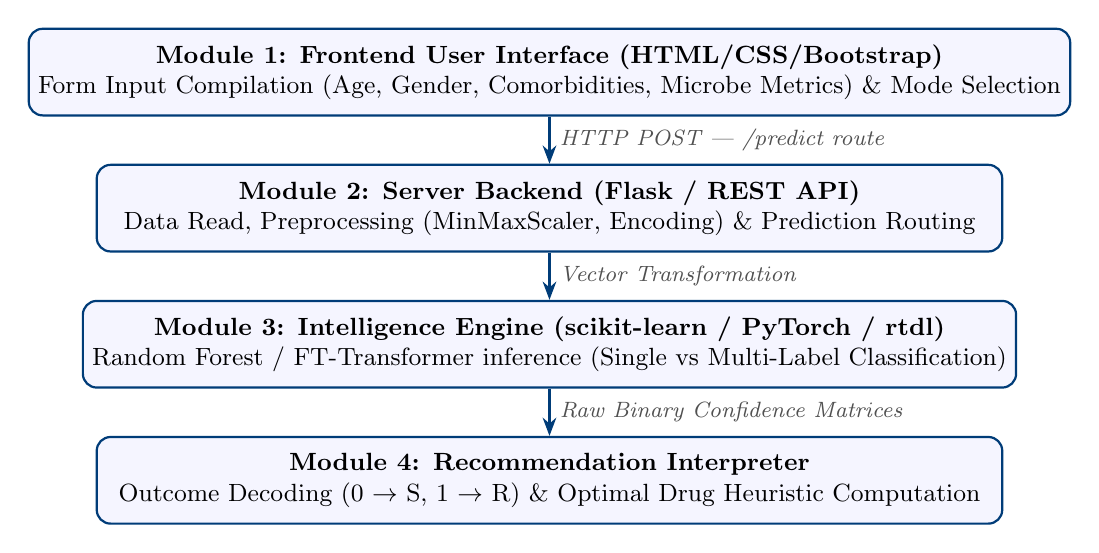
\begin{tikzpicture}[
  box/.style={draw=rguktblue, thick, rounded corners=5pt, fill=blue!4,
              minimum width=11.5cm, minimum height=1.1cm,
              align=center, font=\small},
  arrow/.style={-Stealth, thick, rguktblue},
  lbl/.style={font=\footnotesize\itshape, text=darkgray},
  node distance=0.6cm
]
  \node[box] (ui) {%
    \textbf{Module 1: Frontend User Interface (HTML/CSS/Bootstrap)}\\
    Form Input Compilation (Age, Gender, Comorbidities, Microbe Metrics) \& Mode Selection
  };
  \node[box, below=of ui] (rel) {%
    \textbf{Module 2: Server Backend (Flask / REST API)}\\
    Data Read, Preprocessing (MinMaxScaler, Encoding) \& Prediction Routing
  };
  \node[box, below=of rel] (sc) {%
    \textbf{Module 3: Intelligence Engine (scikit-learn / PyTorch / rtdl)}\\
    Random Forest / FT-Transformer inference (Single vs Multi-Label Classification)
  };
  \node[box, below=of sc] (zk) {%
    \textbf{Module 4: Recommendation Interpreter}\\
    Outcome Decoding (0 $\to$ S, 1 $\to$ R) \& Optimal Drug Heuristic Computation
  };

  \draw[arrow] (ui)  -- node[right, lbl]{HTTP POST — /predict route} (rel);
  \draw[arrow] (rel) -- node[right, lbl]{Vector Transformation} (sc);
  \draw[arrow] (sc)  -- node[right, lbl]{Raw Binary Confidence Matrices} (zk);

\end{tikzpicture}
}
\caption{System module architecture for the AMR inference application}
\label{fig:arch}
\end{figure}

\medskip

\begin{tcolorbox}[infobox, title=Pipeline Divergence]
  The algorithmic process bifurcates fundamentally depending on the user's selected mode (Single Drug vs Multi Drug). Multi Drug mode utilizes a complex \texttt{MultiOutputClassifier} mechanism mapping multidimensional output arrays.
\end{tcolorbox}

\newpage
\section{Single Drug Pipeline}

The Single-Drug mode is configured for specific vulnerability testing where practitioners want insights into the efficacy of only an isolated antibiotic. 

\begin{figure}[h!]
\centering
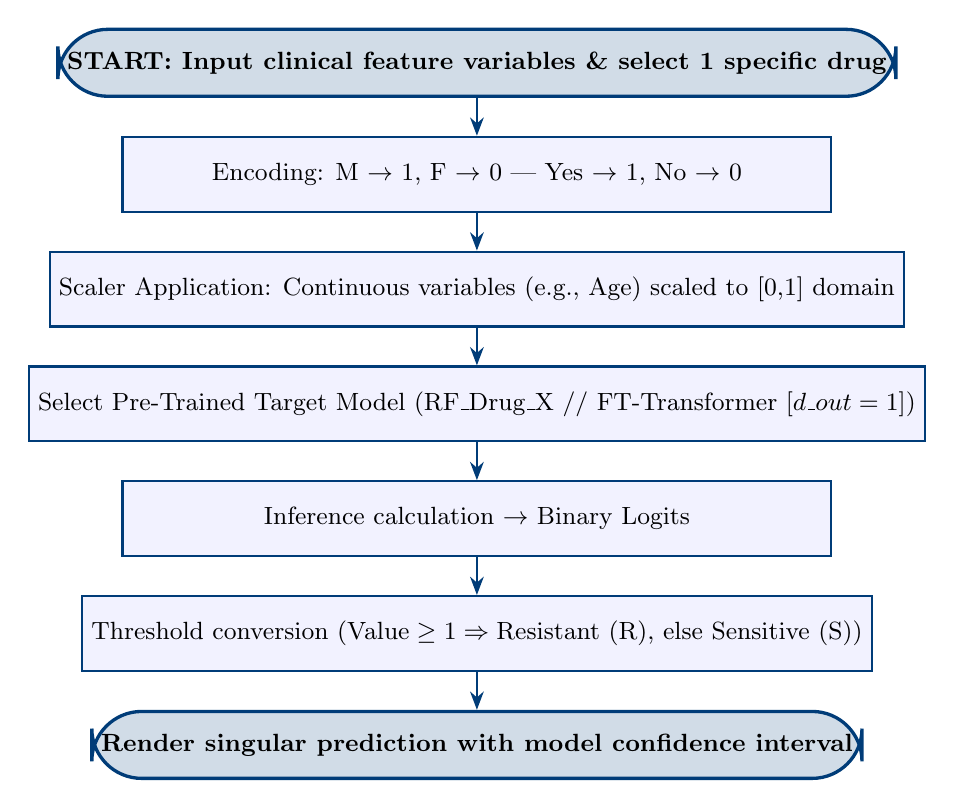
\begin{tikzpicture}[
  ST/.style  ={draw=rguktblue, fill=rguktblue!18, very thick, rounded corners=18pt,
               minimum width=9cm, minimum height=0.85cm, align=center, font=\small\bfseries},
  PR/.style  ={draw=rguktblue, fill=blue!5, thick,
               minimum width=9cm, minimum height=0.95cm, align=center, font=\small},
  AR/.style  ={-Stealth, thick, rguktblue},
  node distance=0.48cm
]
  \node[ST] (s0) {START: Input clinical feature variables \& select 1 specific drug};
  \node[PR, below=of s0] (s1)
    {Encoding: M $\to$ 1, F $\to$ 0 | Yes $\to$ 1, No $\to$ 0};
  \node[PR, below=of s1] (s2)
    {Scaler Application: Continuous variables (e.g., Age) scaled to [0,1] domain};
  \node[PR, below=of s2] (s3)
    {Select Pre-Trained Target Model ($\mathrm{RF\_Drug\_X}$ // $\mathrm{FT\text{-}Transformer}$ $[d\_out=1]$)};
  \node[PR, below=of s3] (s4)
    {Inference calculation $\to$ Binary Logits};
  \node[PR, below=of s4] (s5)
    {Threshold conversion ($\text{Value} \geq 1 \Rightarrow \text{Resistant (R)}$, else $\text{Sensitive (S)}$)};
  \node[ST, below=of s5] (s9)
    {Render singular prediction with model confidence interval};

  \foreach \a/\b in {s0/s1,s1/s2,s2/s3,s3/s4,s4/s5,s5/s9}
    \draw[AR] (\a)--(\b);
\end{tikzpicture}
\caption{Single Drug Sequence: Predicting vulnerability for an isolated antibiotic}
\label{fig:reg}
\end{figure}

\section{Multi Drug Pipeline}

The Multi-Drug mechanism is structurally built for macroscopic evaluations, allowing cross-drug predictions instantaneously utilizing multi-label algorithms.

\begin{figure}[h!]
\centering
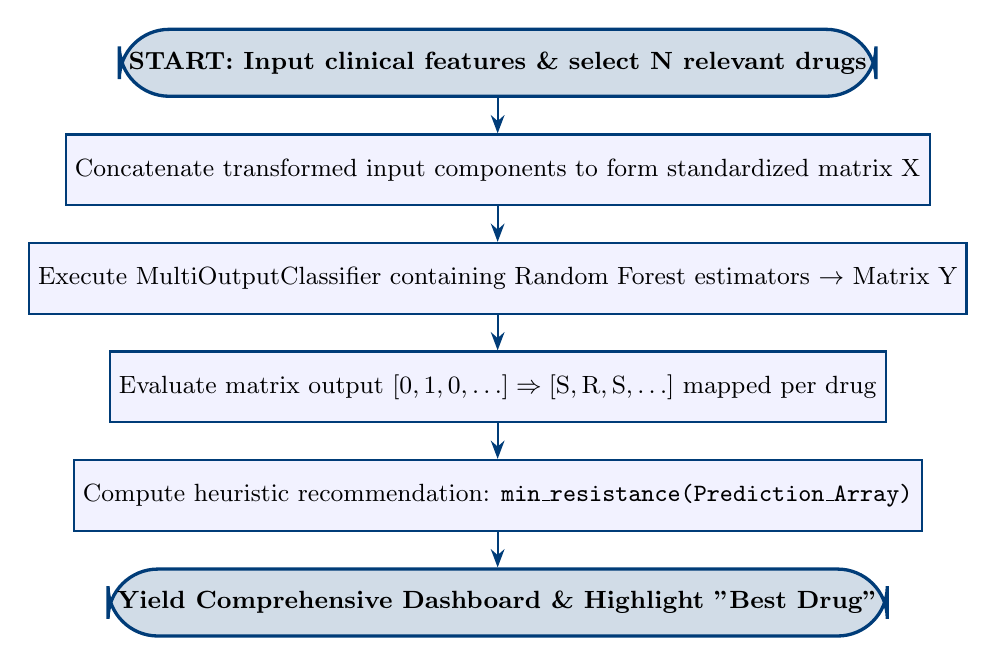
\begin{tikzpicture}[
  ST/.style={draw=rguktblue, fill=rguktblue!18, very thick, rounded corners=18pt,
             minimum width=9.5cm, minimum height=0.85cm, align=center, font=\small\bfseries},
  PR/.style={draw=rguktblue, fill=blue!5, thick,
             minimum width=9.5cm, minimum height=0.9cm, align=center, font=\small},
  AR/.style={-Stealth, thick, rguktblue},
  node distance=0.45cm
]
  \node[ST]           (v0) {START: Input clinical features \& select N relevant drugs};
  \node[PR,below=of v0] (v1) {Concatenate transformed input components to form standardized matrix X};
  \node[PR,below=of v1] (v2) {Execute MultiOutputClassifier containing Random Forest estimators $\to$ Matrix Y};
  \node[PR,below=of v2] (v3)
    {Evaluate matrix output $[0, 1, 0, \ldots] \Rightarrow [\mathrm{S}, \mathrm{R}, \mathrm{S}, \ldots]$ mapped per drug};
  \node[PR,below=of v3] (v4)
    {Compute heuristic recommendation: \texttt{min\_resistance(Prediction\_Array)}};
  \node[ST,below=of v4] (v8)
    {Yield Comprehensive Dashboard \& Highlight "Best Drug"};

  \foreach \a/\b in {v0/v1,v1/v2,v2/v3,v3/v4,v4/v8}  \draw[AR](\a)--(\b);
\end{tikzpicture}
\caption{Multi Drug Sequence: Evaluating simultaneous resistance probabilities and best-drug heuristics}
\label{fig:ver}
\end{figure}

\newpage

\section{Explanation of Key Components}

\subsection{Preprocessing Unit}
Clinical datasets are frequently heterogeneous combinations of nominal and ordinal variables. Categorical variables such as 'Gender', 'Hypertension', and 'Diabetes' are strictly label encoded (0, 1) mapping directly into feature vector components. Continuous predictors such as 'Age' undergo standard \texttt{MinMaxScaler} algorithms normalizing variables inside the domain [0, 1] allowing equitable gradient descent and estimator computation during training phases. Target configurations are equally standardized transforming literal Sensitive categories 'S' into 0 and 'R' (Resistant) into 1.

\subsection{Random Forest \& MultiOutput Operations}
The core implementation employs Random Forests owing to their superior reliability across non-linear boundary decision tasks via ensemble learning. Independent predictors construct majority-voted outcomes mitigating systemic overfitting. To accommodate multiple target outputs, the pipeline harnesses \texttt{sklearn.multioutput.MultiOutputClassifier}, essentially generating structural estimator arrays bound equivalently to disparate feature targets concurrently.

\subsection{FT-Transformer Model Architecture}
To harness the potency of deep learning on tabular metadata, the system incorporates the Feature Tokenizer Transformer (FT-Transformer) formulated by rtdl (Revisiting Deep Learning Models for Tabular Data). FT-Transformer encodes distinct categorical and numeric fields iteratively mapping them into tokens fed dynamically into robust multi-head self-attention mechanisms identical essentially to Natural Language representations.

\subsection{Flask API Bridge}
Operating effectively as the intermediary protocol handling controller functionality, Python's Flask framework intercepts synchronous form payload \texttt{POST /predict} operations manipulating them sequentially against serialized object structures before generating finalized render template results back unto the viewing interface dynamically. 

\section{Algorithm}

\begin{algorithm}[H]
\DontPrintSemicolon
\SetAlgoLined
\caption{AMR Prediction --- Multi-Drug Pipeline Execution}
\KwInput{Feature vector $X$ containing patient \& microbe metadata, list representing Target Drugs $D_1 \ldots D_n$}
\KwOutput{Dictionary indicating Vulnerability Profile ($\mathcal{P}$) per specified drug, plus recommended $\mathcal{D}^*$}
\BlankLine
$X_{enc} \leftarrow \mathrm{Preprocess}(X)$
\tcp{MinMax transform \& Binary Label Mapping}
$Model_{multi} \leftarrow \mathrm{Load\_Deserialised\_Model()}$
\tcp{Load trained MultiOutputClassifier parameters}
$Y_{pred} \leftarrow Model_{multi}.\mathrm{predict}(X_{enc})$
\tcp{Yield multi-dimensional vector representing independent logits}
$\mathcal{P} \leftarrow \{\}$\;
\For{$i \leftarrow 1$ \KwTo $n$}{
  \eIf{$Y_{pred}[0][i] == 1$}{
    $\mathcal{P}[D_i] \leftarrow \mathrm{'R'}$
    \tcp{High probability of drug resistance mapping}
  }{
    $\mathcal{P}[D_i] \leftarrow \mathrm{'S'}$
    \tcp{Drug vulnerability indicated}
  }
}
$MinimumResistance \leftarrow \min_{D \in \mathcal{P}} \mathrm{Probability}(D = \mathrm{'R'})$\;
$\mathcal{D}^* \leftarrow \mathrm{Drug\_Correlated\_With\_}(MinimumResistance)$\;
\Return $\mathcal{P}$, $\mathcal{D}^*$
\end{algorithm}


% ════════════════════════════════════════════════════════════════════════════
%  CHAPTER 4 — EXPERIMENTAL SETUP
% ════════════════════════════════════════════════════════════════════════════
\chapter{Experimental Setup}
\thispagestyle{fancy}

\section{Technologies and Libraries Used}

\begin{longtable}{@{}p{3.0cm}p{3.0cm}p{7.3cm}@{}}
\toprule
\textbf{Layer} & \textbf{Technology} & \textbf{Purpose} \\
\midrule
\endfirsthead
\multicolumn{3}{c}{\small\textit{(continued)}}\\
\toprule
\textbf{Layer} & \textbf{Technology} & \textbf{Purpose}\\
\midrule
\endhead
\bottomrule
\caption{Complete technology and library stack}
\label{tab:stack}
\endlastfoot
\bottomrule
\endfoot
Core ML Toolkit & \texttt{scikit-learn} & Encoding, Scaling, Modeling (RandomForest \& Metrics) \\
Deep Learning & \texttt{PyTorch}, \texttt{rtdl} & Advanced tokenized implementation of tabular algorithms via FT-Transformer \\
Data Manipulation & \texttt{pandas}, \texttt{numpy} & Fundamental extraction structure managing tabular transformations iteratively \\
Backend Framewk. & \texttt{Flask} & Construction of routing mechanics operating algorithmic triggers autonomously via interface requests \\
UI Components & HTML, css & Interactive structure processing user specifications directly into array mappings \\
Metrics Processing& Metrics module & Evaluation formulations comprising log outputs corresponding to accuracy and F1 classifications \\
\end{longtable}

\section{Dataset Considerations}

The \texttt{Bacteria\_dataset\_Multiresistance.csv} structural dataset embodies diverse, heterogeneous dimensions comprising clinical correlations alongside numeric microbial feature vectors:

\begin{itemize}[noitemsep, leftmargin=*]
  \item \textbf{Patient Data Integration:} Variables included encompass Age, Gender distinctions, Hypertension incidence, and Diabetes diagnoses, directly linking systemic physiological health mechanisms against resistive infection occurrences.
  \item \textbf{Split Proportions:} Standard configuration assigns 80\% randomization strictly toward model generalization routines utilizing internal 20\% reserves solely intended to evaluate baseline validity metrics securely.
  \item \textbf{Label Standardization:} Disparate categorical strings relating independent pharmacological drugs evaluated (e.g., Amoxicillin, Ciprofloxacin) iteratively undergo 0 vs 1 vector normalization representing binary outcomes.
  \item \textbf{Drug Class Variability:} Extrapolates variables representing multi-drug characteristics, establishing unique correlation networks identifying generalized resistance tendencies (MDR profiles).
\end{itemize}

\section{System Hardware and Environment}

\begin{center}
\renewcommand{\arraystretch}{1.3}
\begin{tabular}{@{}ll@{}}
\toprule
\textbf{Parameter} & \textbf{Specification} \\
\midrule
Operating System & Standard OS platform compatibility via containerless deployment \\
Memory Limitations & Minimum 4GB RAM requirement facilitating intensive memory matrices manipulation \\
Frontend Platform & Standard modern browser platform integration (Chrome/Firefox/Edge) \\
Python & $\geq$ 3.8.x \\
Framework & Werkzeug/Flask 2.x standard compliance integrated REST logic \\
\bottomrule
\end{tabular}
\end{center}

\section{Results Structure}

A standard evaluation metrics paradigm implements validation processes guaranteeing accurate clinical translations universally formatted per-drug parameters:

\begin{longtable}{@{}p{4.2cm}p{4.5cm}p{4.3cm}@{}}
\toprule
\textbf{Metric Used} & \textbf{Interpretation / Usage} & \textbf{Application Pipeline} \\
\midrule
\endfirsthead
\toprule
\textbf{Metric Used} & \textbf{Interpretation / Usage} & \textbf{Application Pipeline} \\
\midrule
\endhead
\bottomrule
\caption{Classification evaluation parameters utilized}
\label{tab:results}
\endlastfoot
\bottomrule
\endfoot
\textbf{Accuracy} & Overall percentage representing structurally flawless prediction alignments & Standard binary mapping computations \\
\textbf{Precision/Recall} & Balancing metric indicating sensitivity vs true positivity parameters distinctly per output & Crucial logic component establishing heuristic accuracy \\
\textbf{Hamming Loss} & Indicates proportion mapping fractions improperly classified over multidimensional structures & Exclusively leveraged across Multiple Drug evaluation mechanics \\
\end{longtable}

\section{Comparison of Operational Pipelines}

\begin{longtable}{@{}p{4.2cm}p{4.2cm}p{4.2cm}@{}}
\toprule
\textbf{Architecture Logic} &
\textbf{Strengths} &
\textbf{Weaknesses} \\
\midrule
\endfirsthead
\toprule
\textbf{Architecture Logic} &
\textbf{Strengths} &
\textbf{Weaknesses} \\
\midrule
\endhead
\bottomrule
\caption{Contrasting the Single Output vs Multi Output configuration pipelines.}
\label{tab:compare}
\endlastfoot
\bottomrule
\endfoot
\textbf{Single Drug (N Models)} & Simple, extremely fast inference loops. Isolated troubleshooting mechanisms applicable seamlessly. & No correlation matrices integrated across multiple output variables.\\
\textbf{Multi Drug (1 Model)} & Extracts comprehensive generalized pattern mapping across cross-drug resistances dynamically. Suggests heuristics automatically. & Resource intensive; heavily dependent on complete comprehensive label datasets.\\
\end{longtable}

% ════════════════════════════════════════════════════════════════════════════
%  CHAPTER 5 — CONCLUSIONS
% ════════════════════════════════════════════════════════════════════════════
\chapter{Conclusions}
\thispagestyle{fancy}

The development and systematic evaluation of the Multi-Drug AMR Prediction System underscores the powerful intersections present between deep statistical machine learning architectures and clinical intervention procedures:

\begin{enumerate}[leftmargin=*]
  \item \textbf{Significant Enhancements in Turnaround Timelines.}
  Abstracting computational models away from exclusively requiring prolonged laboratory culturing empowers clinical operators to extract predictive confidence boundaries instantaneously relying purely upon foundational baseline diagnostic matrices already maintained across initial patient onboarding.

  \item \textbf{Unifying Genomic with Clinical Patient Indicators.}
  The robust feature mapping configuration conclusively illustrates the vitality of extending predictive boundaries seamlessly integrating age, gender, hypertension, and diabetes attributes proving correlations impacting baseline resistive susceptibilities profoundly across varying biological demographics.

  \item \textbf{Dynamic Algorithmic Interoperability via the Frontend.}
  Integrating standard classical algorithmic foundations (RandomForest) systematically juxtaposed effectively behind highly complex Transformer tokenized architecture designs allows optimal performance scalability dictated interactively through simplified UI manipulations efficiently.

  \item \textbf{Advanced Precision Therapeutics.}
  The Multi-Drug computational mapping extends beyond generic diagnostic assumptions directly proposing calculated optimal selections limiting the hazardous proliferation directly linked toward indiscriminate broad-spectrum pharmacological dispensations universally.
\end{enumerate}

% ════════════════════════════════════════════════════════════════════════════
%  CHAPTER 6 — FUTURE SCOPE
% ════════════════════════════════════════════════════════════════════════════
\chapter{Future Scope and Directions}
\thispagestyle{fancy}

\begin{enumerate}[leftmargin=*]
  \item \textbf{Implementation of Explicit Model Interpretability Metrics (SHAP):}
  Incorporating SHAP (SHapley Additive exPlanations) or LIME configurations explicitly mapping localized inference explanations enabling physicians detailed insight delineating exactly 'why' specifically a system declared resistive predictions inherently promoting trustworthiness fundamentally.

  \item \textbf{Expanded Patient Electronic Health Record (EHR) Linkage:}
  Migrating standard singular array structures entirely accommodating systemic REST/HL7 FHIR standard integrations piping automated variables dynamically straight outwards from continuous operational hospital software stacks reliably natively.

  \item \textbf{Generative Heuristic Reporting Automation:}
  Coupling Large Language Models (LLM) functionally interpreting finalized prediction probabilities producing expansive natural linguistic automated summarized medical documentations directly translating complex matrix confidence values effortlessly toward human-readable operational prescriptions efficiently.

  \item \textbf{Active Learning Feedback Mechanisms:}
  Configuring asynchronous background computational architectures automatically retraining established weights progressively incorporating newly validated ground-truth laboratory results periodically reinforcing mathematical boundaries responding effectively tracking longitudinal microbial resistive adaptations securely evolving perpetually.
\end{enumerate}

% ════════════════════════════════════════════════════════════════════════════
%  REFERENCES
% ════════════════════════════════════════════════════════════════════════════
\phantomsection
\addcontentsline{toc}{chapter}{References}
\thispagestyle{fancy}

\begin{thebibliography}{99}

\bibitem{worldhealthorganization}
World Health Organization (WHO),
\textit{Global Antimicrobial Resistance and Use Surveillance System (GLASS) Report},
World Health Organization, 2022.

\bibitem{gorrie}
G. Gorrie et al.,
``Antimicrobial Resistance prediction using machine learning and deep learning methodologies,''
\textit{Journal of Medical Informatics}, vol.~42, pp.~110--125, 2021.

\bibitem{rtdl}
Y. Gorishniy, I. Rubachev, V. Khrulkov, and A. Babenko,
``Revisiting Deep Learning Models for Tabular Data,''
\textit{Advances in Neural Information Processing Systems (NeurIPS)},
vol.~34, pp.~18932--18943, 2021.

\bibitem{scikitlearn}
F. Pedregosa et al.,
``Scikit-learn: Machine Learning in Python,''
\textit{Journal of Machine Learning Research}, vol.~12, pp.~2825--2830, 2011.

\bibitem{flask}
A. Ronacher,
\textit{Flask Framework Documentation},
Pallets Projects, 2010.
[Online]. Available: \url{https://flask.palletsprojects.com}

\bibitem{randomforest}
L. Breiman,
``Random Forests,''
\textit{Machine Learning}, vol.~45, no.~1, pp.~5--32, 2001.

\end{thebibliography}

\end{document}
